\chapter{Data Stratification}
\label{chapter:data_stratification}


In order to better understand the properties of the data in the \ac{iemo} dataset, we performed stratification based on several attributes of the dataset. The aim of this stratification was to group similar data together and investigate their common properties, and, discover limitations that these properties pose to the machine learning model in the \ac{ser} area.

\section{Recordings Durations}

The duration of an audio recording can significantly impact the analysis and modeling of the data. Shorter recordings may not capture enough information to adequately represent the signal of interest, while longer recordings may contain irrelevant or redundant information.

We stratified the dataset based on the duration of the recordings. The dataset contains recordings ranging from approximately 0.25 to 33 seconds in duration, and we divided the recordings into three groups: short, less than or equal to 2.5 seconds, medium, greater than 2.5 and less than or equal to 4.5 seconds, and long, greater than 4.5 seconds.

Table \ref{5:durations} presents the impact of the duration of the recordings on the performance of the chosen traditional AdaBoost model. The longest recordings have the highest performance, with an accuracy of 63.4\%, despite having more recordings than the medium duration data. 

\begin{table}[H]
	\centering
	\caption{Traditional Model 5-Fold Cross-Validation Results Based on the Recordings Duration.}
	\label{5:durations}
	\begin{tabular}{lrlrrrr}
		\toprule
		Recordings Duration &   Total Data & Accuracy    &   Macro F1 &   Precision &   Recall &   MCC. \\
		\midrule
		Short ($]0, 2.5]$ s)	&         2103 & 56.54+-1.5  &      54.85 &       58.49 &    53.47 &   0.39 \\
		Medium ($]2.5, 4.5]$ s)	& 		  1674 & 56.87+-0.82 &      57.17 &       57.79 &    57.09 &   0.42 \\
		Long ($]4.5, 34]$ s)	&         1754 & 63.4+-2.28  &      63.77 &       64.25 &    63.67 &   0.51 \\
		\bottomrule
	\end{tabular}
\end{table}

These results suggest that longer recordings provide more information and are easier for the model to classify accurately, which allows us to conclude that recordings' duration has a significant performance impact on the \ac{ser} task.

\section{Speaker Gender}

Another attribute we used for stratification was the gender of the speaker. The dataset contains a similar amount of recordings from both male and female speakers, having 2649 recordings with female speakers and 2882 with male speakers.

To evaluate the performance of the model on different genders, we trained and tested the model on recordings from female speakers, male speakers, and mixed-gender recordings. Table \ref{5:gender} shows the 5-fold cross-validation results of the model on each category.

\begin{table}[H]
	\centering
	\caption{Traditional Model 5-Fold Cross-Validation Results Based on Speaker Gender Recordings.}
	\label{5:gender}
	\begin{tabular}{llrrrrr}
		\toprule
		Training Gender & Testing Gender & Accuracy    &   Macro F1 &   Precision &   Recall &   MCC. \\
		\midrule
		Female	& Female & 59.87+-1.03 & 60.45 & 60.55 & 60.77 & 0.46 \\
		Male 	& Male	 & 59.92+-1.33 & 60.43 & 61.66 & 59.72 & 0.45 \\
		Female  & Male	 & 51.49+-1.38 & 51.55 & 53.67 & 51.52 & 0.33 \\
		Male    & Female & 51.45+-1.76 & 52.01 & 55.35 & 51.23 & 0.35 \\
		\bottomrule
	\end{tabular}
\end{table}

From the table, it can be observed that the model performed similarly on both genders, when the testing data for the model is of the training data, with accuracies close to 60\%. However, when testing with different speaker gender, the model's accuracy dropped significantly to 51.49\% and 51.45\% for female and male training data, respectively. The other metrics showed equivalent behavior, indicating difficulty in correctly identifying the emotion in mixed-gender contexts.

These results suggest that the model's performance is affected by the gender of the speakers in the training data and that the model is biased toward it.


\section{Discrete Emotions}

The \ac{iemo} dataset contains four emotional categories: anger, happiness, sadness, and neutral. We stratified the data based on these labels and obtained 15 groups of data. In this section, we discuss the differences in classification performance between these emotional categories, as well as differences in valence and emotional plane.


Table \ref{tab:emo_cat} shows the traditional model 5-fold cross-validation results based on the discrete emotions. In the four-label case, which includes all four emotional categories, the model achieved an accuracy of 60.04\% with a macro F1 score of 60.76. The best performance was achieved when classifying between anger, happiness, and sadness, with an accuracy of 70.36\% and a macro F1 score of 70.73. The worst performance was achieved when classifying between angry, neutral, and happy, with an accuracy of 64.4\% and a macro F1 score of 63.8.


\begin{table}[H]
\small
\centering
\caption{Traditional Model 5-Fold Cross-Validation Results Based on the Discrete Emotions.}
\label{tab:emo_cat}
    \centering
    \begin{tabular}{lrrrrrr}
    	\toprule
    	Labels                      &   Total Data & Accuracy    & Macro F1    & Precision   & Recall      & MCC.       \\
    	\midrule
 	    \multicolumn{7}{c}{Four Labels} \\
    	Angry, Happy, Sad, Neutral             &         5531 &  60.04$\pm$0.95 & 60.76 & 61.29 & 60.59 & 0.459 \\
    	\midrule
    	\multicolumn{7}{c}{Three Labels} \\
    	
		Angry, Happy, Sad                   &         3823 & 70.36$\pm$1.09 &      70.73 &       71.36 &    70.35 &   0.54 \\
		Angry, Neutral, Happy               &         4447 & 64.4$\pm$0.95  &      63.8  &       64.48 &    63.84 &   0.46 \\
		Angry, Neutral, Sad                 &         3895 & 74.02$\pm$1.14 &      74.16 &       75.61 &    73.2  &   0.6  \\
		Sad, Neutral, Happy                 &         4428 & 65.4$\pm$1.12  &      65.59 &       65.75 &    65.54 &   0.47 \\
		
		Sad, Neutral, Happy+Angry (Arousal) &         5531 & 68.54$\pm$1.03 &      66    &       66.31 &    65.89 &   0.49 \\
		Angry+Sad, Neutral, Happy (Valence) &         5531 & 60.15$\pm$0.86 &      58.94 &       59.53 &    58.99 &   0.39 \\
    	\midrule
    	\multicolumn{7}{c}{Two Labels} \\
    	    	
    	Angry, Sad                          &         2187 & 91.4$\pm$1.46  &      91.4  &       91.46 &    91.39 &   0.83 \\
    	Angry, Neutral                      &         2811 & 84.13$\pm$0.88 &      82.98 &       84.03 &    82.34 &   0.66 \\
    	Angry, Happy                    &         2739 & 74.66$\pm$2.01 &      73.1  &       73.84 &    72.72 &   0.47 \\
    	Sad, Neutral                        &         2792 & 79.51$\pm$1.57 &      77.98 &       78.77 &    77.49 &   0.56 \\
    	Sad, Happy                          &         2720 & 83.6$\pm$1.41  &      82.87 &       82.93 &    82.82 &   0.66 \\
    	Neutral, Happy                      &         3344 & 72.58$\pm$2.38 &      72.43 &       72.81 &    72.45 &   0.45 \\
    	Sad+Neutral, Happy+Angry (Arousal)  &         5531 & 77.2$\pm$1.29  &      77.18 &       77.25 &    77.18 &   0.54 \\
    	Angry+Sad, Neutral+Happy (Valence)  &         5531 & 72.86$\pm$0.94 &      69.84 &       72.47 &    69.27 &   0.42 \\
    	\bottomrule
    \end{tabular}
\end{table}

In the two-label case, where the emotional categories were paired, the best performance was achieved when classifying between angry and sad, with an accuracy of 91.4\% and a macro F1 score of 91.4. The worst performance was achieved when classifying between angry+sad and neutral+happy based on valence, with an accuracy of 72.86\% and a macro F1 score of 69.84.

In terms of valence and emotional plane, the model achieved its highest accuracy (68.54\%) when classifying between sad, neutral, and happy+angry based on arousal, and its lowest accuracy (60.15\%) when classifying between angry+sad, neutral, and happy based on valence. These results suggest that the model is better at distinguishing emotional categories based on arousal than valence.

It is important to note that the total data impacts the classification, as a lower number of files may make the classification easier. However, even with a large dataset such as \ac{iemo}, the performance of the model varied widely depending on the emotional categories and valence or arousal being classified. These results have implications for the development of affective computing systems, which must take into account the nuances of emotional categorization and valence/arousal classification in order to accurately interpret and respond to human affect.


\section{Dimensional Emotions}

In addition to the categorical classification discussed in the previous section, we also explored dimensional classification using the annotations of the dataset in terms of valence (ranging from unpleasant to pleasant), arousal (ranging from calm to excited), and dominance (ranging from submissive to dominant). These annotations are provided by human annotators who rate each recording on three continuous dimensions, on a scale from 1 to 5.



\begin{table}[H]
	\centering
	\caption{Discrete Emotions' Means of the Dimensional Annotations.}
	\label{tab:dis_dim}
	\begin{tabular}{lrrr}
		\toprule
		Emotion & Mean Activation &   Mean Valence & Mean Dominance \\
		\midrule
		Angry   &   3.636 &  1.906 &  3.949 \\
		Happy   &   3.411 &  3.946 &  3.228 \\
		Neutral &   2.726 &  2.971 &  2.831 \\
		Sad     &   2.564 &  2.253 &  2.828 \\
		\bottomrule
	\end{tabular}
\end{table}




Our results suggest that the valence and arousal dimensions are easier to classify than the dominance dimension. One possible reason for this is that dominance is a more complex and abstract concept that may be more difficult to recognize and classify in speech. Additionally, the annotations for dominance may be more subjective and varied among annotators than those for valence and arousal, leading to less reliable labels and lower classification performance.

Overall, our results demonstrate the potential of using dimensional classification in speech emotion recognition. Future work could explore the use of more advanced machine learning models and feature extraction techniques to improve the performance of the model on the dominance dimension and to further investigate the relationship between acoustic features and the three dimensions of emotion.




\begin{figure}[H]
  \centering
  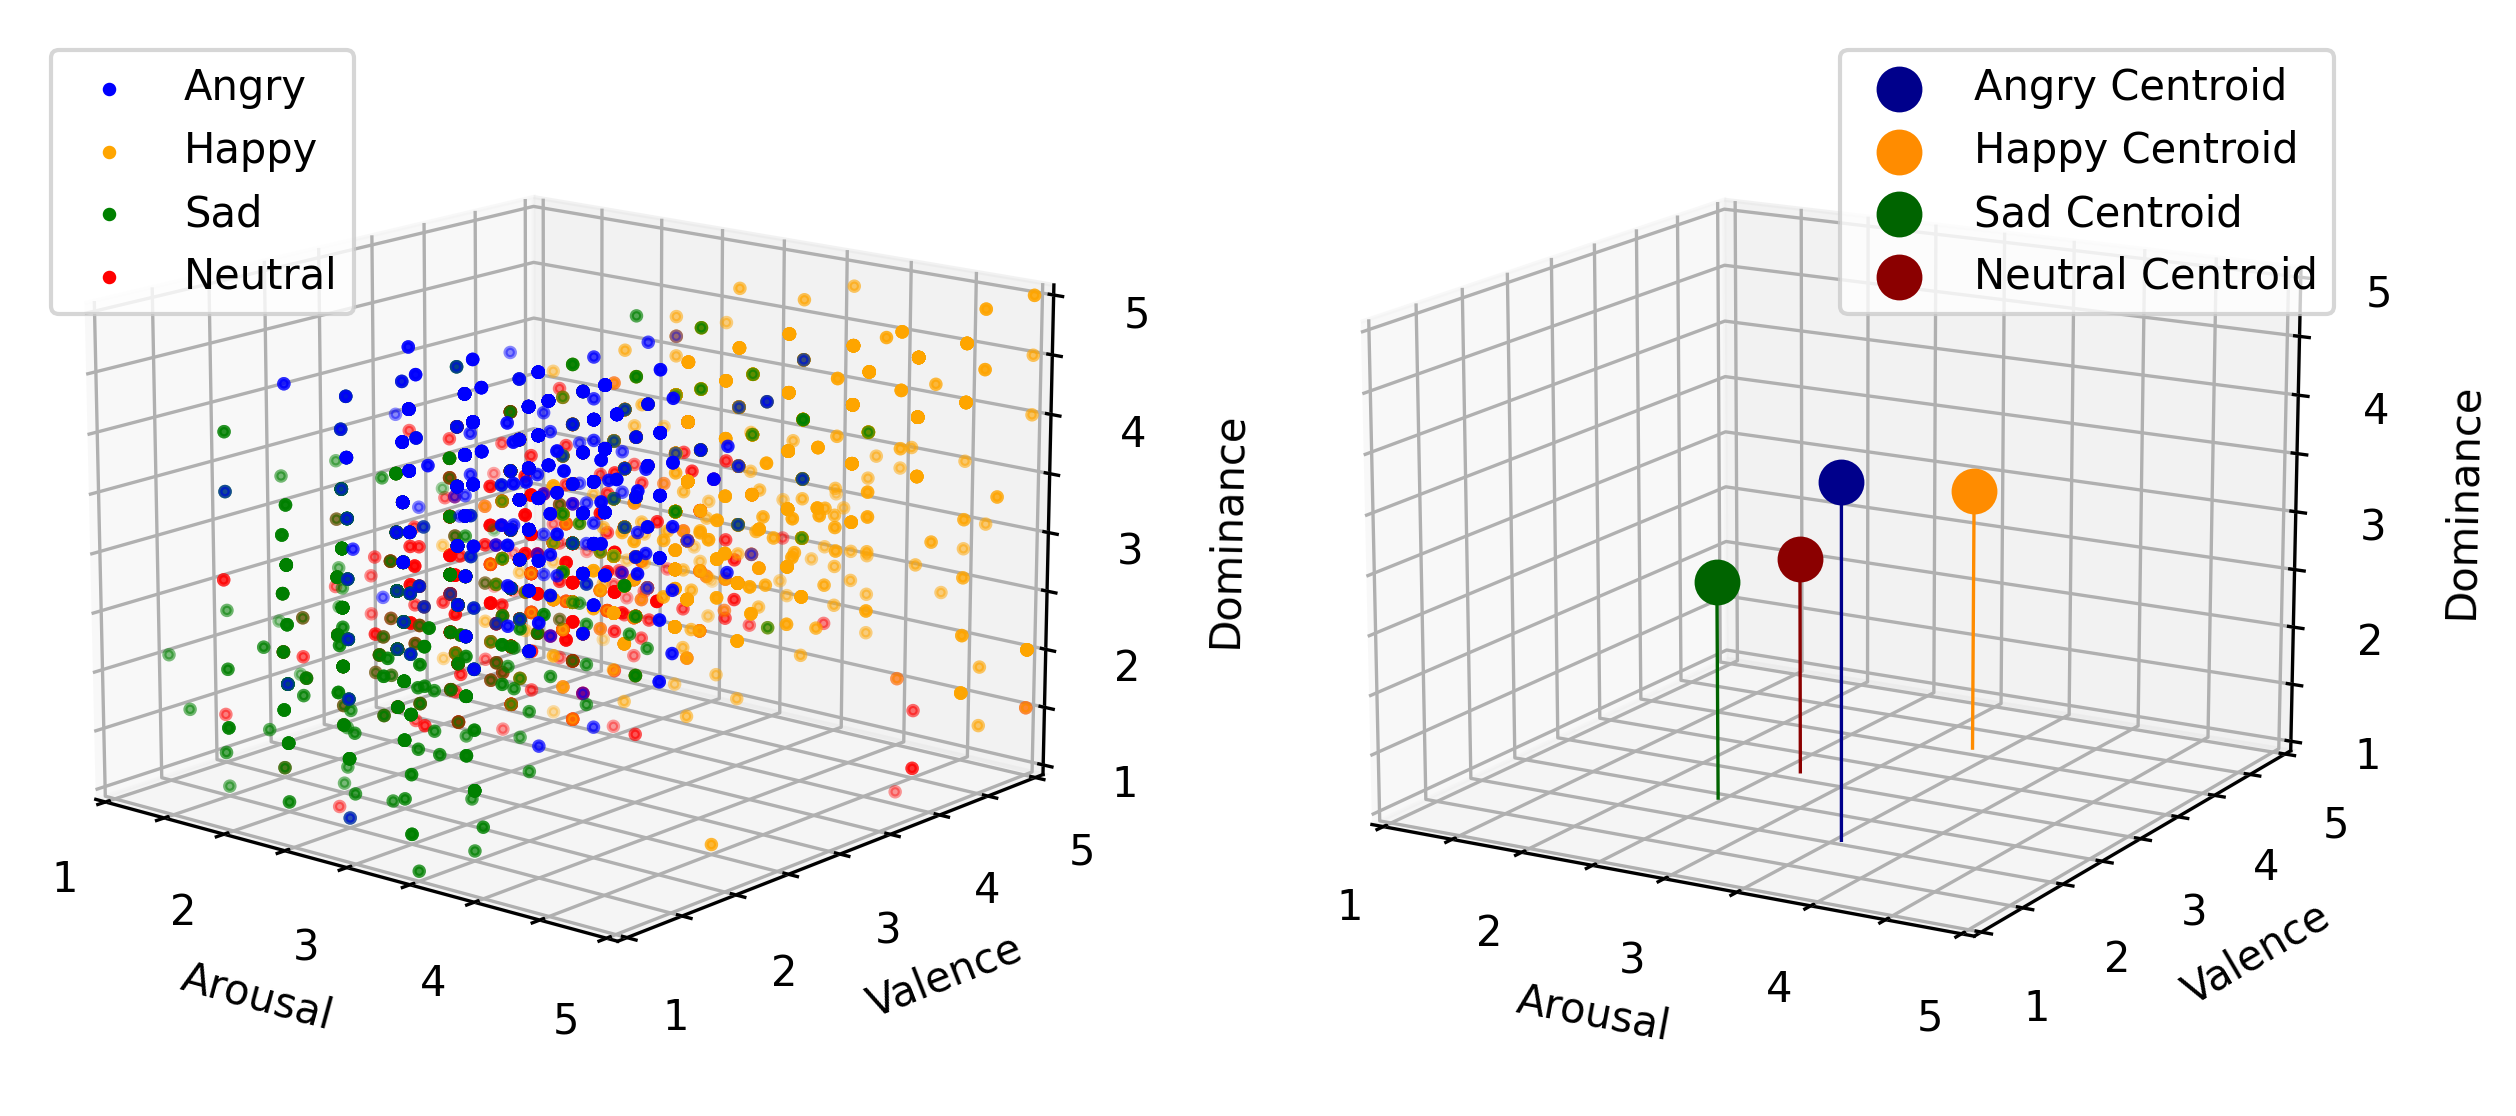
\includegraphics[width=.9\linewidth]{figs/5_data_stratification/primitives_visualization.png}
  \caption{Juries dimensional emotion classifications 3D visualization}
  \label{fig:signalWP}
\end{figure}

\begin{figure}[H]
  \centering
  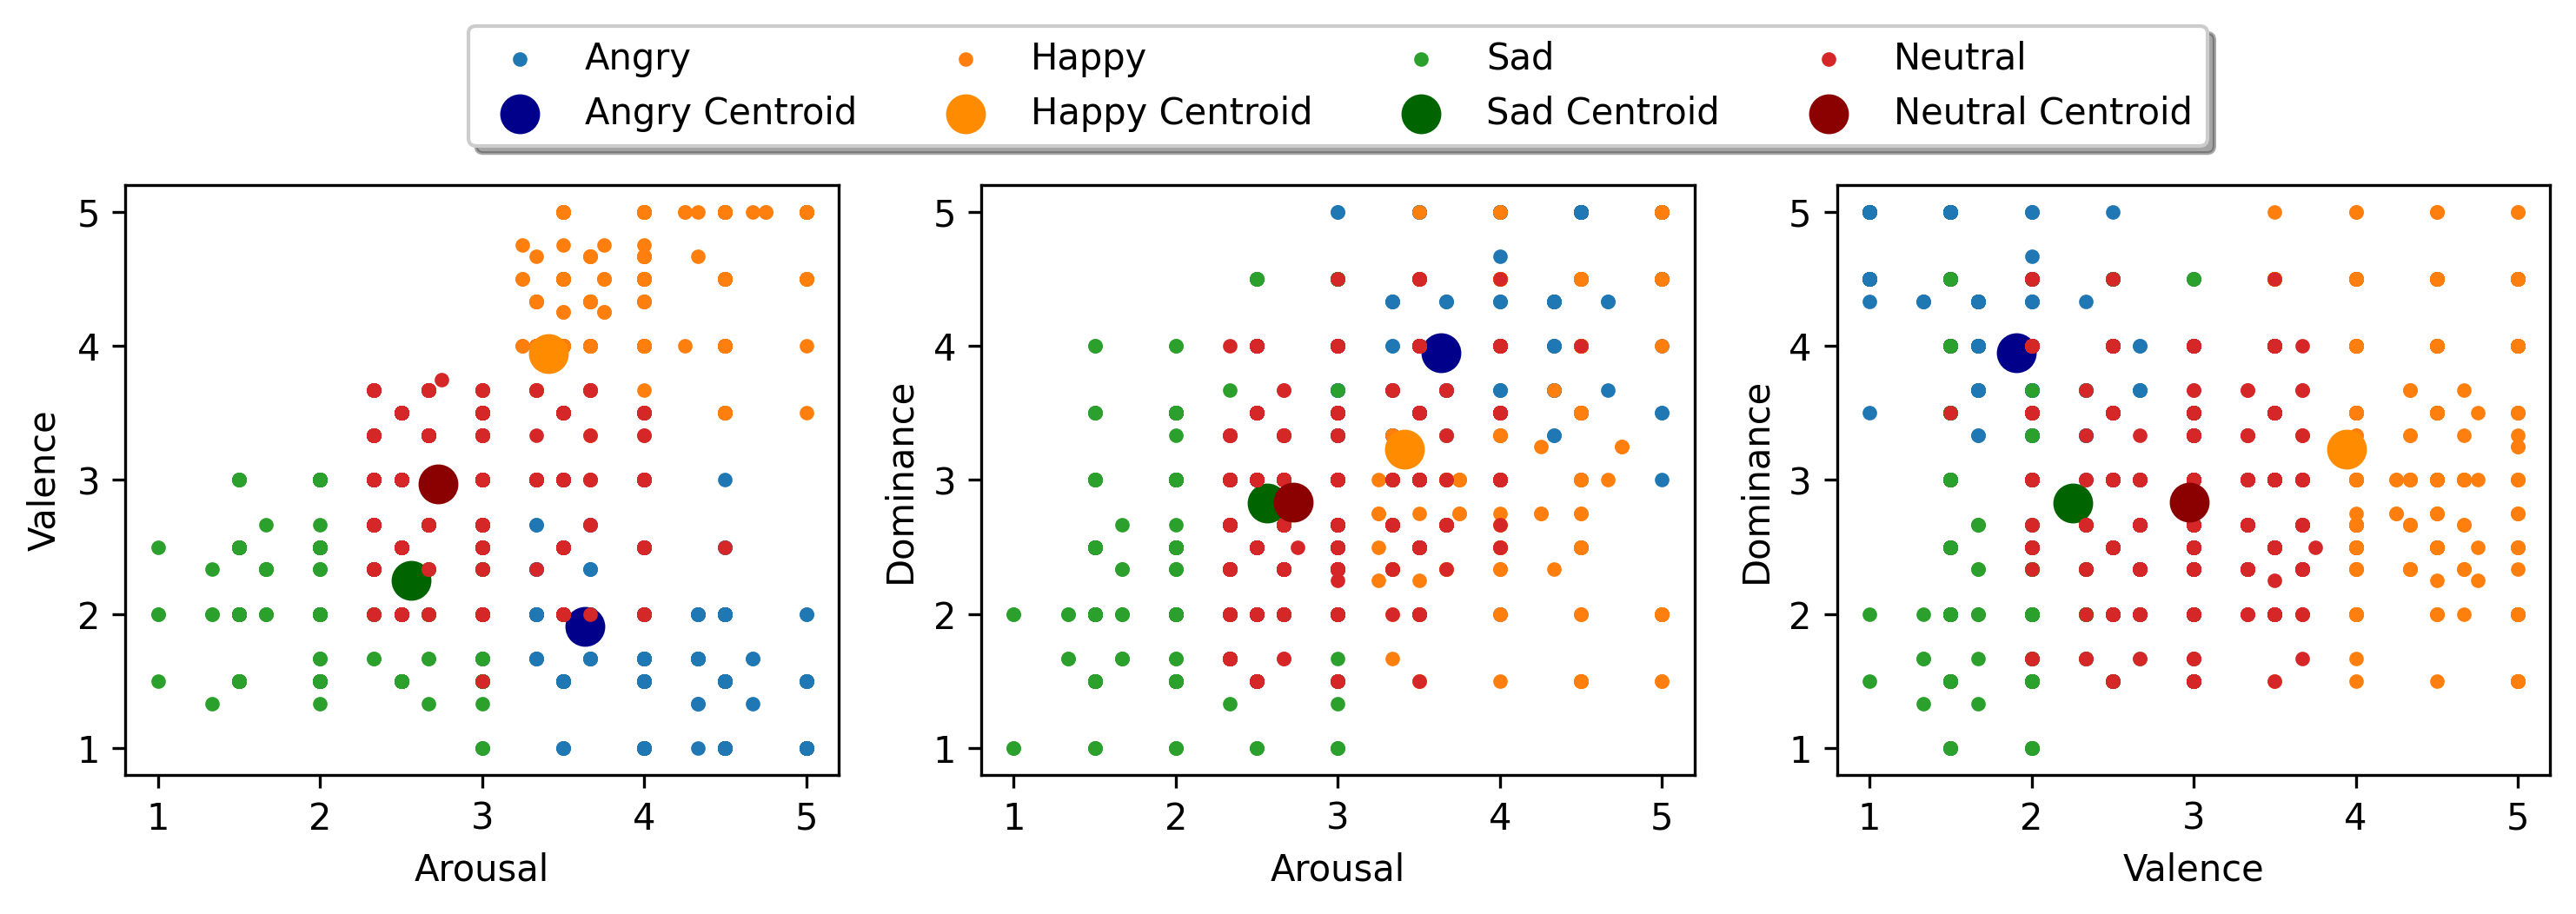
\includegraphics[width=.9\linewidth]{figs/5_data_stratification/primitives_visualization_2d.png}
  \caption{Juries dimensional emotion classifications 2D visualization}
  \label{fig:signalWP}
\end{figure}


CITE CONFLICTS FROM THIS https://ieeexplore.ieee.org/document/9746930:

TODO: NAO MOSTRAR OS CONFLITOS RETIRADOS MAS SIM MOSTRAR OS RANGES MANTIDOS

\begin{table}[H]
\caption{Conflicts between emotion's categories and primitives}
\label{tab:dominance}
\centering
    \begin{tabular}{lrrr}
        \toprule
        {} & \multicolumn{3}{c}{\textbf{Conflicts}} \\ \cmidrule{2-4}
        Emotion Categories &    Arousal &      Valence &       Dominance \\
        
        \addlinespace
        \hline
        \multicolumn{4}{c}{\cellcolor{gray!15}{\textbf{Non-Strict Conflicts}}} \\
        \hline
        \addlinespace
        
        Angry   &    $[1, 2.5]$ & $]3.5, 5]$ & $[1, 2[$ \\         \addlinespace
        Happy+Excited &  $[1, 3[$  & $[1, 3[$ & $[1, 2[$ \\   \addlinespace
        Sad    &    $[3.5, 5]$ & $[3.5, 5]$ & None \\         \addlinespace
        Neutral  &  $[1, 2[$ & $]4, 5]$ & $[1, 1.5[ \cup ]4.5, 5]$\\ 

        \addlinespace
        \hline
        \multicolumn{4}{c}{\cellcolor{gray!15}{\textbf{Strict Conflicts}}} \\
        \hline
        \addlinespace

        Angry   &    $[1, 3]$ &  $[3, 5]$ &  $[1, 2[$ \\         \addlinespace
        Happy+Excited &  $[1, 3]$ & $[1, 3]$ & $[1, 2[$ \\   \addlinespace
        Sad    &   $[4, 5]$ & $[4, 5]$ & None  \\         \addlinespace
        Neutral  &  $[1, 2]$ & $[4, 5]$ & $[1, 2[ \cup ]4, 5]$ \\

        \bottomrule
    \end{tabular}
\end{table}



\begin{figure}[H]
  \centering
  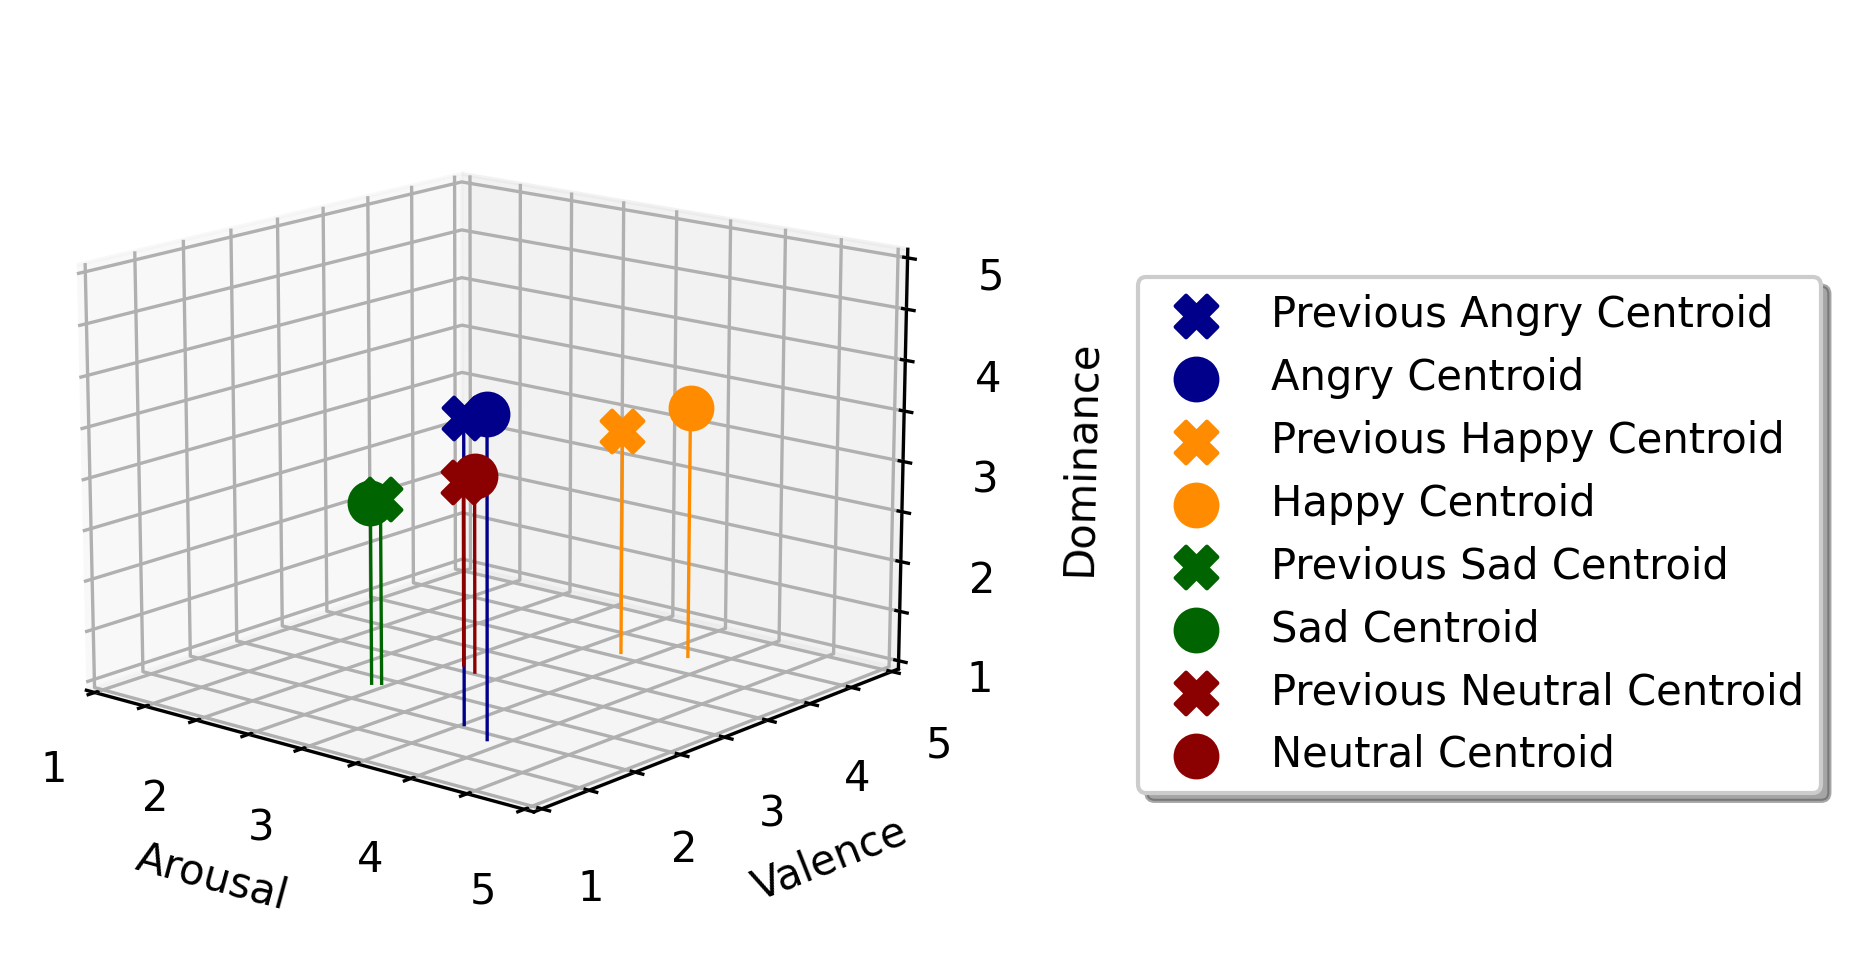
\includegraphics[width=.9\linewidth]{figs/5_data_stratification/strict_conflicts_centroids.png}
  \caption{Data with and without conflicts between emotion's categories and primitives emotion centroids' 3D visualization}
  \label{fig:signalWP}
\end{figure}

\begin{figure}[H]
  \centering
  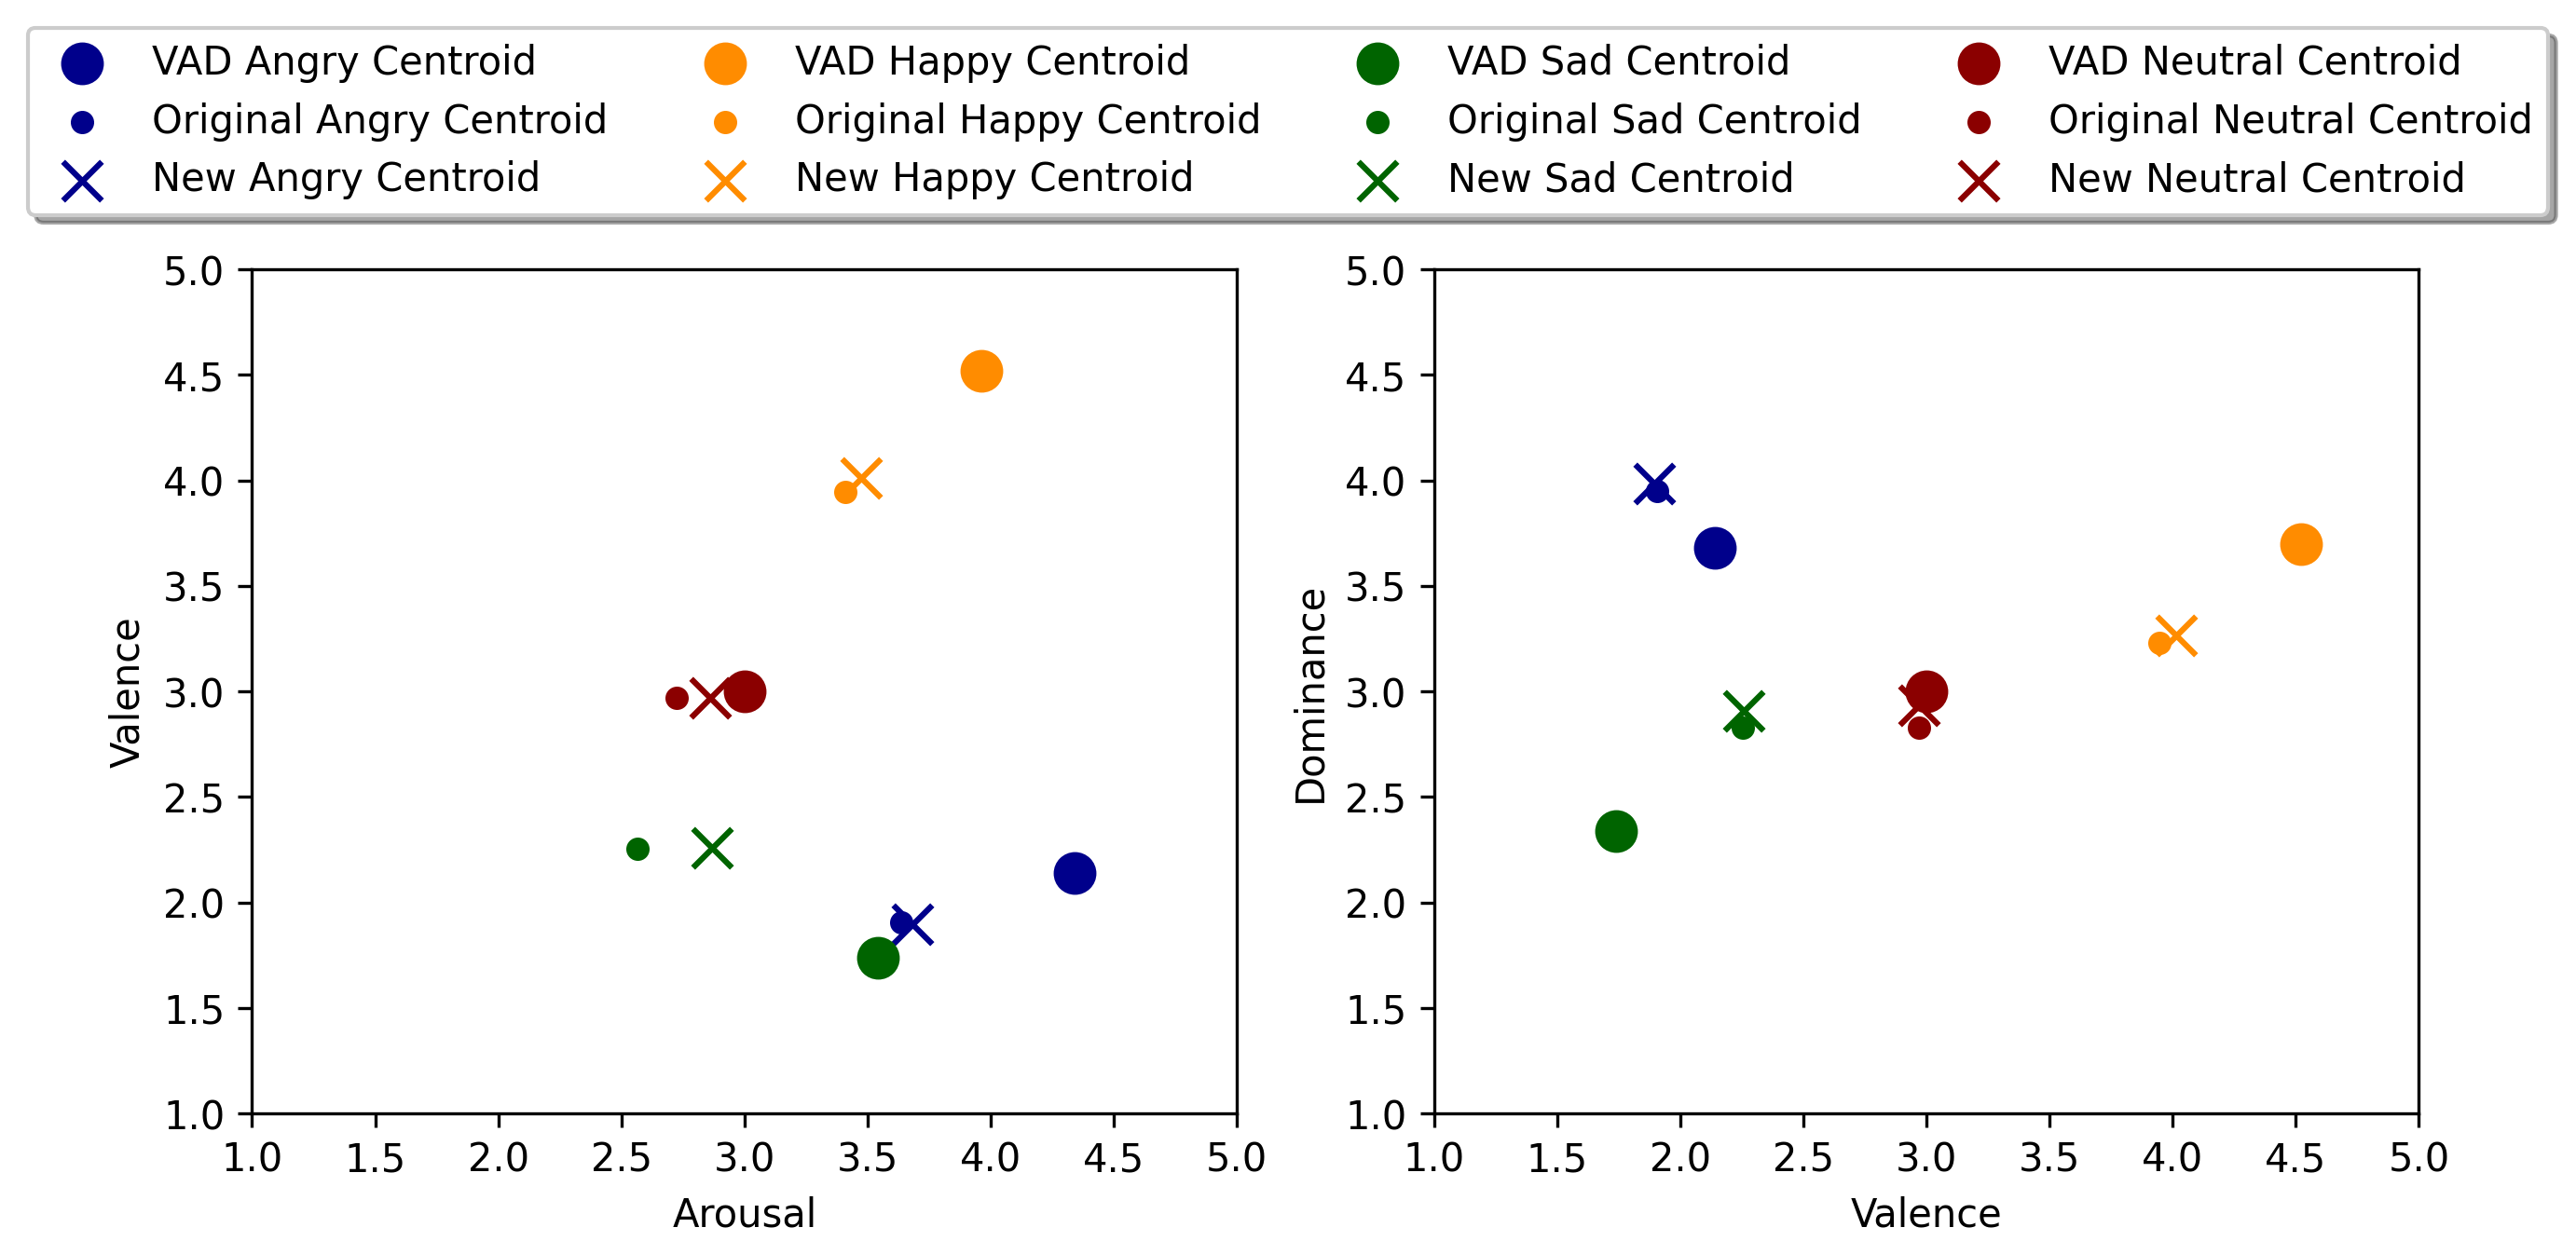
\includegraphics[width=.9\linewidth]{figs/5_data_stratification/strict_conflicts_centroids_2d.png}
  \caption{Data with and without conflicts between emotion's categories and primitives emotion centroids' 2D visualization}
  \label{fig:signalWP}
\end{figure}



\begin{table}[H]
\small
\caption{Results obtained after eliminating emotions based on VAD conflicts with the categorical annotations.}
\label{tab:dominance}
\centering
    \begin{tabular}{lrr}
        \toprule
        Conflicts Removed &    Total Data &  Accuracy  \\
        \midrule
        None & 5531 & 60.26+-0.46 \\         \addlinespace
        
        \hline
        \addlinespace
        
        Non-strict Arousal    &   4955 & 63.37+-1.09 \\         \addlinespace
        Non-strict Valence    &  5382 &  60.46+-0.95 \\   \addlinespace
        Non-strict Dominance   & 5491  & 60.5+-0.93 \\         \addlinespace
        All Non-strict  &  4816 & 65.05+-0.85 \\         \addlinespace
        
        \hline
        \addlinespace
        
        Strict Arousal    &  4222 & 66.79+-1.85 \\         \addlinespace
        Strict Valence    &  5128 &  62.07+-1.77 \\   \addlinespace
        Strict Dominance   & 5432  & 60.53+-1.34 \\         \addlinespace
        All Strict  &  3911 & 69.09+-1.17 \\         \addlinespace
        \bottomrule
    \end{tabular}
\end{table}
